\documentclass[12pt]{article}
\usepackage{graphicx}
\usepackage{float}

\title{CS 496 Assignment 4: Mobile Development}
\author{Ian Kronquist}

\begin{document}
\maketitle

Video URL: http://people.oregonstate.edu/~kronquii/cloudandmobile.mov


If you have problems viewing this video, please let me know ASAP. It may not be viewable from your browser and may need to be downloaded and played in a dedicated video player. It's viewable with QuickTime on OS X.

\section{Mobile Application}
The mobile application is a simple selfie snapper. Users can take a photo with their camera and upload it to Imgur. I then display the URL from the API response so the user can share it. Under the hood I use the Android camera intent and make an asynchronous request to the Imgur upload API.

When the user opens the application they are greeted by some text which says ``Upload a selfie to Imgur''. There are two buttons at the bottom which say ``Take Photo'', and ``Upload to Imgur''. The upload button is initially disabled, since there isn't anything to upload yet.

\begin{figure}[H]
    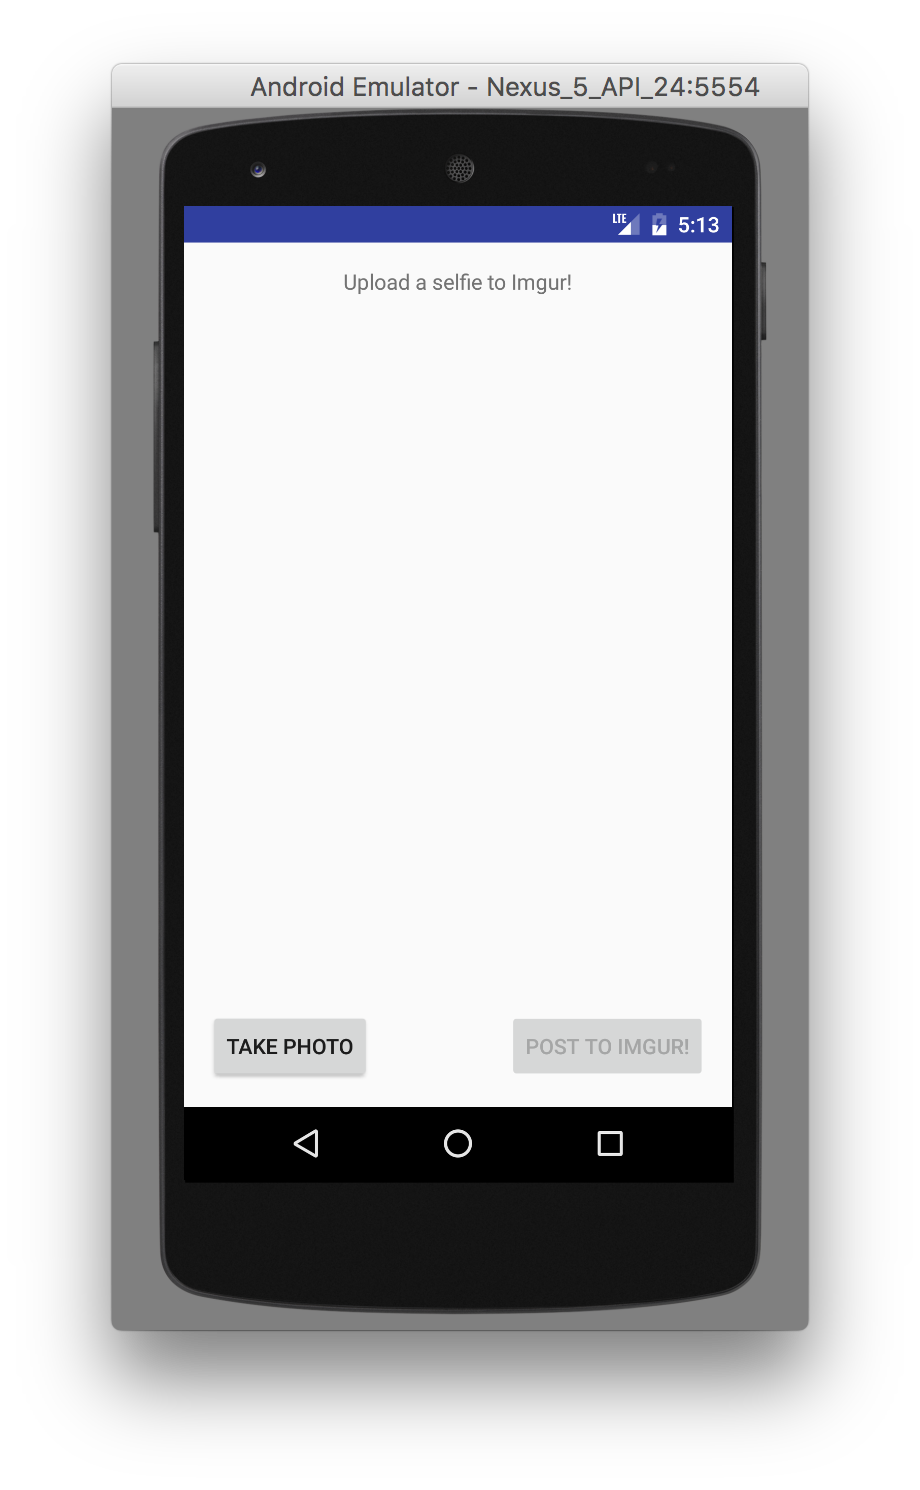
\includegraphics[scale=0.5]{./step1.png}
    \caption{Initial screen}
\end{figure}



When the user presses the upload button, the app transitions to the camera intent. The user can take multiple pictures and decide which one they like best. They can also press the close button and return to the main activity screen. Once they tap the select button it will transition back to the main activity view and display the image in the image view element in the middle of the screen.
\begin{figure}[H]
    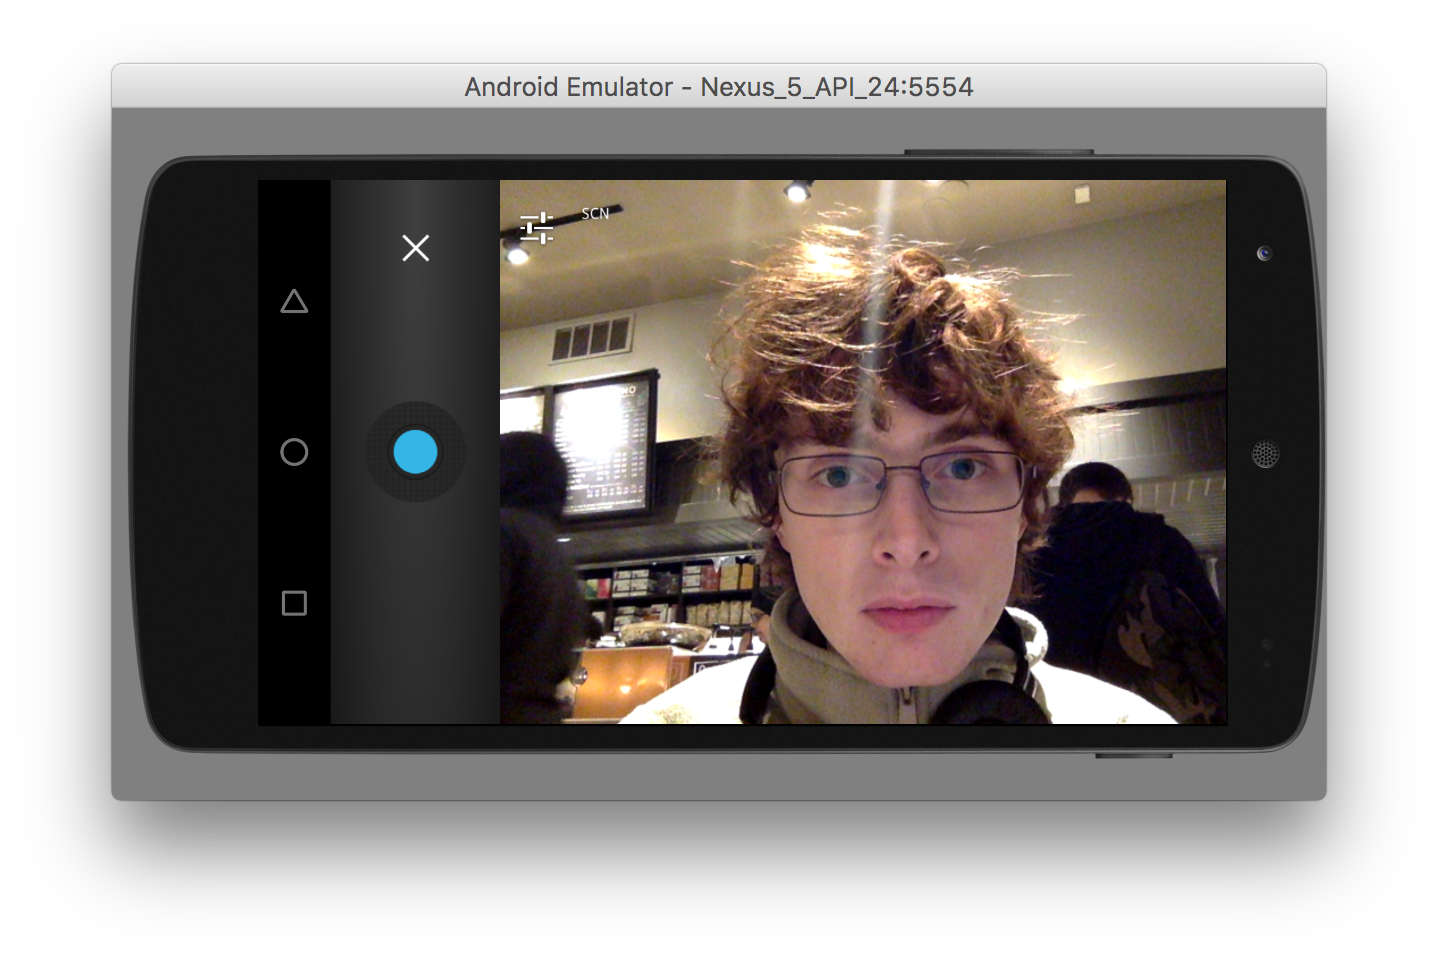
\includegraphics[scale=0.5]{./step2.png}
    \caption{Camera Intent}
\end{figure}


\begin{figure}[H]
    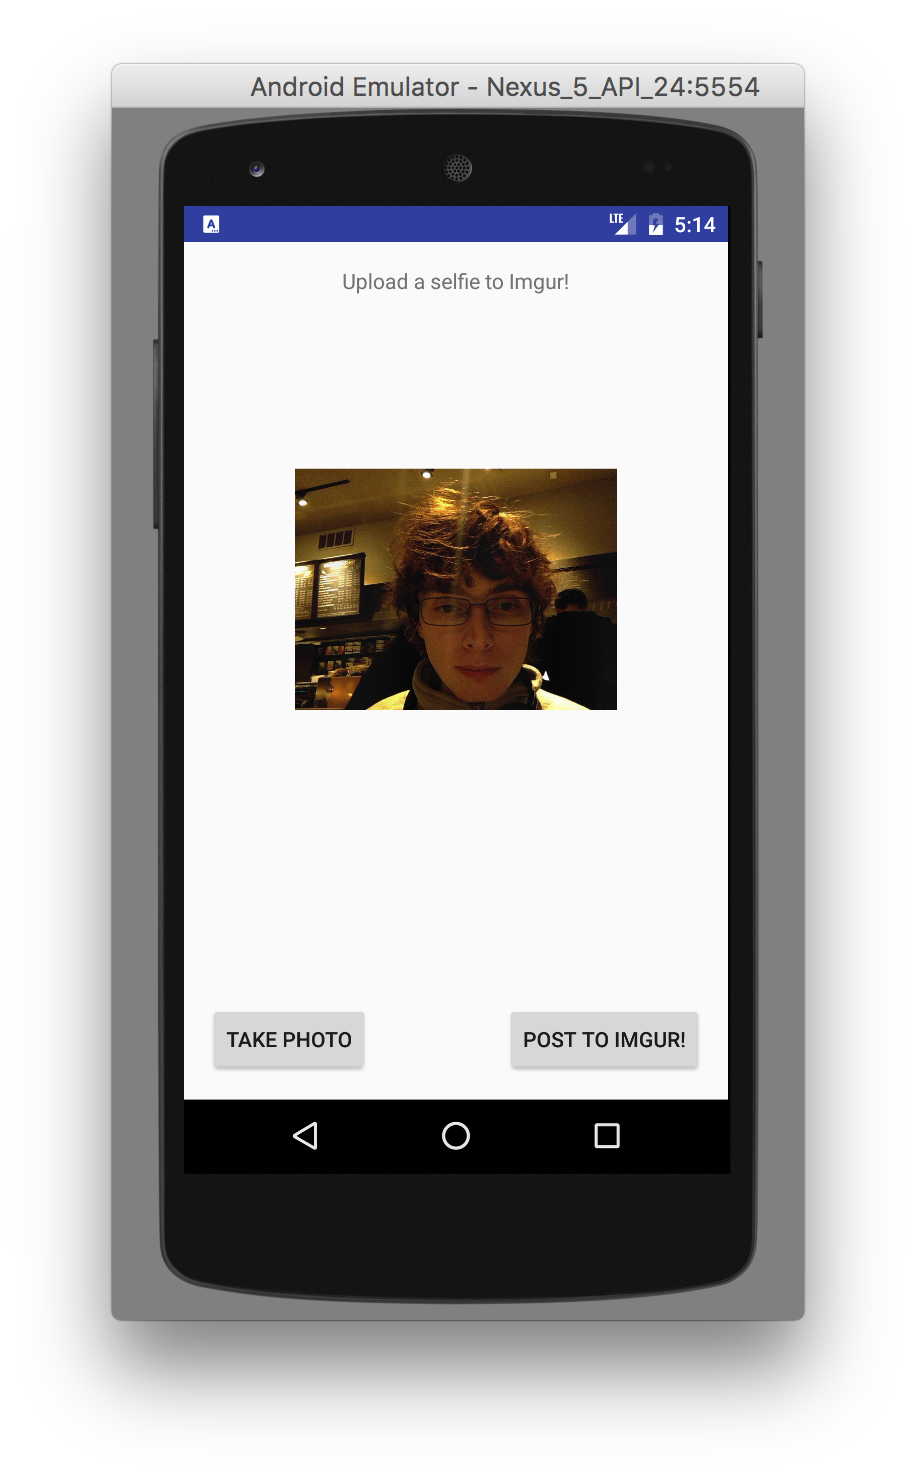
\includegraphics[scale=0.5]{./step3.png}
    \caption{Viewing the image}
\end{figure}


The user can then press the upload button. The application will display a small pop-up known as a Toast to let them know that the work is happening in the background. The upload happens asynchronously so the application is still responsive. When the upload finishes, it will replace the text at the top of the screen with the Imgur URL of their photo, or a message if an error occurred. Users can then go back and reupload the image to get a new URL, or take a new photo and upload it.

\begin{figure}[H]
    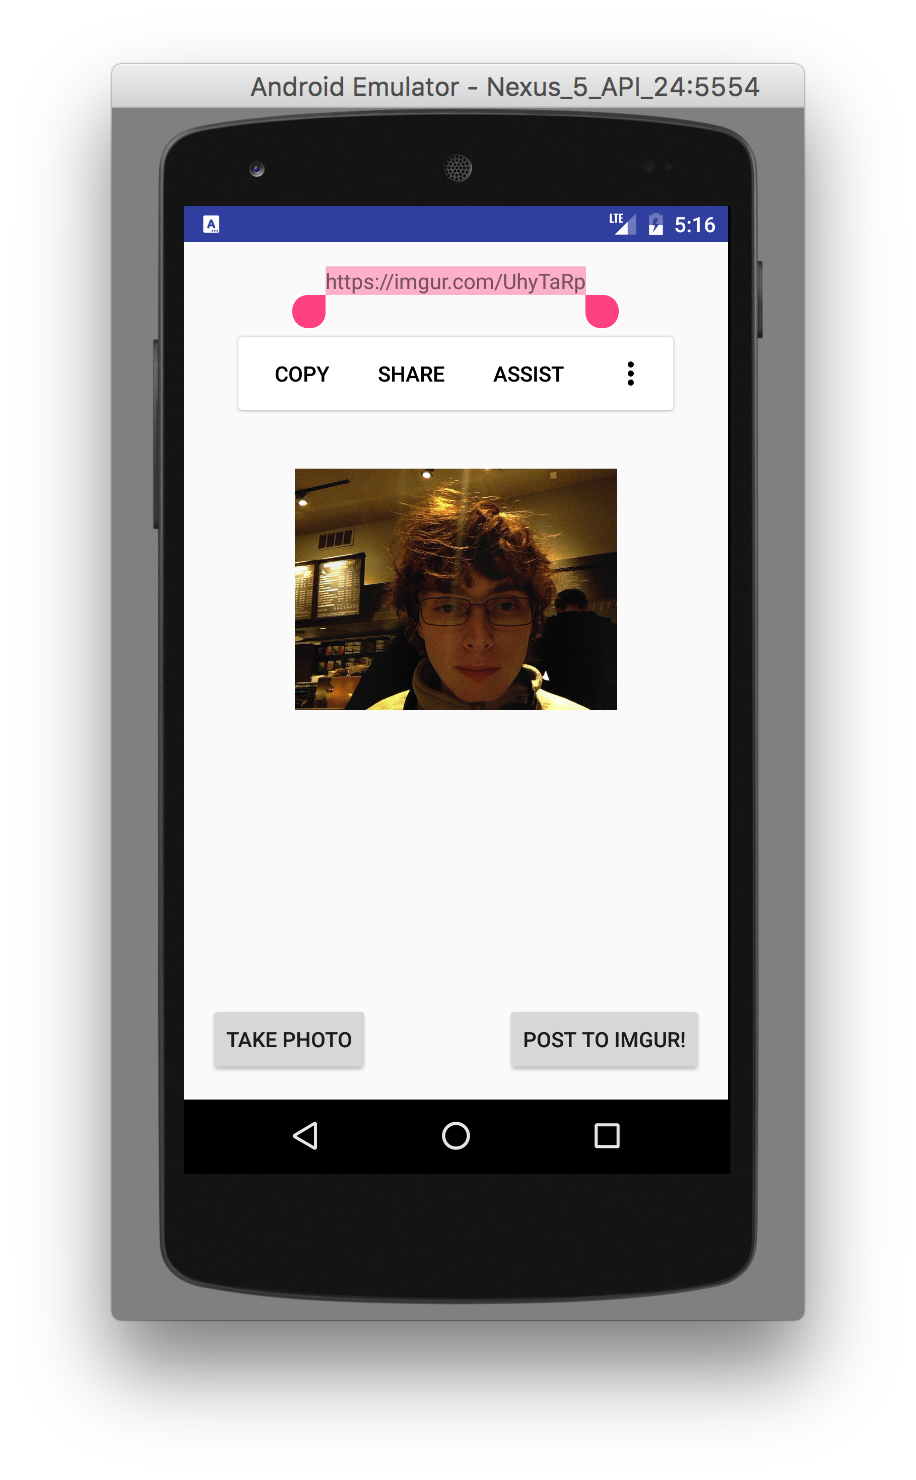
\includegraphics[scale=0.5]{./step4.png}
    \caption{Copying the URL}
\end{figure}


Navigation for the application was a non-issue. The application only has a single activity view, so there was no need to add any functionality to the back button. The user can't view previous images because they are destroyed after being uploaded.

One of the more difficult parts of writing this application was the Android permissions system. In Android M there was an overhaul of the permissions system which required users to grant each permission individually. Many online tutorials and even some of the official documentation didn't make it clear which permissions were required, or how to specifically request them.



\begin{verbatim}
    public void takePhoto(View view) {
        if (checkSelfPermission(Manifest.permission.CAMERA) !=
                PackageManager.PERMISSION_GRANTED ||
                checkSelfPermission(Manifest.permission.WRITE_EXTERNAL_STORAGE) !=
                        PackageManager.PERMISSION_GRANTED) {
            requestPermissions(new String[]{Manifest.permission.CAMERA,
                    Manifest.permission.WRITE_EXTERNAL_STORAGE}, 0);
        }

        try {
            Intent intent = new Intent(MediaStore.ACTION_IMAGE_CAPTURE);
            File photo = new File(Environment.getExternalStorageDirectory(),
                "Pictures/Pic.jpg");
            photo.getParentFile().mkdirs();
            new FileOutputStream(photo).close();
            imageUri = FileProvider.getUriForFile(Act1.this,
                    BuildConfig.APPLICATION_ID + ".provider", photo);
            intent.putExtra(MediaStore.EXTRA_OUTPUT,
                    imageUri);
            startActivityForResult(intent, TAKE_PICTURE);
        } catch (Exception e) {
            e.printStackTrace();
            Toast.makeText(Act1.this, "Uh oh! Looks like we had a problem",
                    Toast.LENGTH_LONG).show();
        }
    }
\end{verbatim}



\section{Imgur API}
The Imgur API was surprisingly easy to use. To make a request, the developer first needs to authenticate themselves with the OAuth2 protocol. They need to set a client ID and a client secret in their request headers they send with the request. Like any good API, Imgur supports several different versions. My application uses the latest version 3.


The Imgur API has a wide variety of endpoints for doing things like uploading images, fetching image metadata, favoriting an image, and refreshing the client secret. Since my app is so simple, I only make a single post request to the \texttt{https://api.imgur.com/3/upload.json} endpoint to upload an image. I include the image in the request as a multipart file. Fortunately, the Android HTTP libraries take care of splitting the image and formatting it as part of the request. I make sure to add the \texttt{Authorization: Client-ID} header and add the API key to the multipart request entity. Finally I execute the HTTP request.

\begin{verbatim}
        protected Boolean doInBackground(String... files) {
            final String upload_to = "https://api.imgur.com/3/upload.json";
            final String API_key = "e4d31dbb14e259fa15db0878bb1ae5def4075fb0";
            final String clientId = "669c016e544468d";

            HttpClient httpClient = new DefaultHttpClient();
            HttpContext localContext = new BasicHttpContext();
            HttpPost httpPost = new HttpPost(upload_to);
            httpPost.addHeader("Authorization", "Client-ID " + clientId);

            try {
                final MultipartEntity entity = new MultipartEntity(
                        HttpMultipartMode.BROWSER_COMPATIBLE);
                File photo = new File(Environment.getExternalStorageDirectory(),
                    "Pictures/Pic.jpg");
                entity.addPart("image", new FileBody(photo));
                entity.addPart("key", new StringBody(API_key));
                httpPost.setEntity(entity);
                final HttpResponse response = httpClient.execute(httpPost,
                    localContext);
\end{verbatim}

The \texttt{HttpClient.execute} method is blocking, and will wait until the request finishes. Fortunately, all of this happens off of the main thread, so the UI will not hang until it receives the response. The \texttt{HttpResponse}'s body is then reacted and parsed as a JSON object. If the HTTP entity response was 200 and that the \texttt{success} property of the JSON object is true, I a string to hold the full URL based on the image ID from the JSON object. However, if the response was not successful, I set it to a useful error message.


\begin{verbatim}
                final String response_string = EntityUtils.toString(response
                        .getEntity());

                final JSONObject json = new JSONObject(response_string);
                Log.d("JSON", "received json object:" + json.toString());

                if (response.getStatusLine().getStatusCode() == 200 &&
                        json.getBoolean("success")) {
                    imageName = "https://imgur.com/" +
                        json.getJSONObject("data").getString("id");
                } else {
                    imageName = "Request failed with status " +
                            response.getStatusLine().getStatusCode() + "
                                and error " +
                            json.getString("error");
                }
                return true;
\end{verbatim}

I also make sure to perform some rather zealous and boring error checking to ensure that the user's experience is not negatively impacted. I try to provide a helpful error message for the user.

\begin{verbatim}
            } catch (Exception e) {
                e.printStackTrace();
                Toast.makeText(Act1.this,
                    "Oops, couldn't upload the image!" +
                    " Make sure you're connected to the internet and try again",
                        Toast.LENGTH_LONG).show();
                Log.d("PostFailure", "failed to do something " + e.toString());
                return false;
            }
        }
\end{verbatim}



\end{document}
